\section{Delivered Image Quality and PSF}
\label{sec:delivered_image_quality_and_psf}


Image quality and PSF modeling are closely tied to the progress of the AOS system, and here is what can be concluded halfway through the data gathering with LSSTComCam. \\

\textbf{On Image Quality:} \\

The best image quality achieved so far is 0.7 arcsec, with a median of 1.1 arcsec during science visits. As shown in Table \ref{tab:psf_summary} and Figure \ref{seeing_plot}, the PSF FWHM as a function of observation dates highlights the progress. It is important to note that all these data were collected during the AOS testing and validation phase. This makes the achieved image quality even more encouraging, demonstrating significant progress.

\begin{figure*}
        \centering
        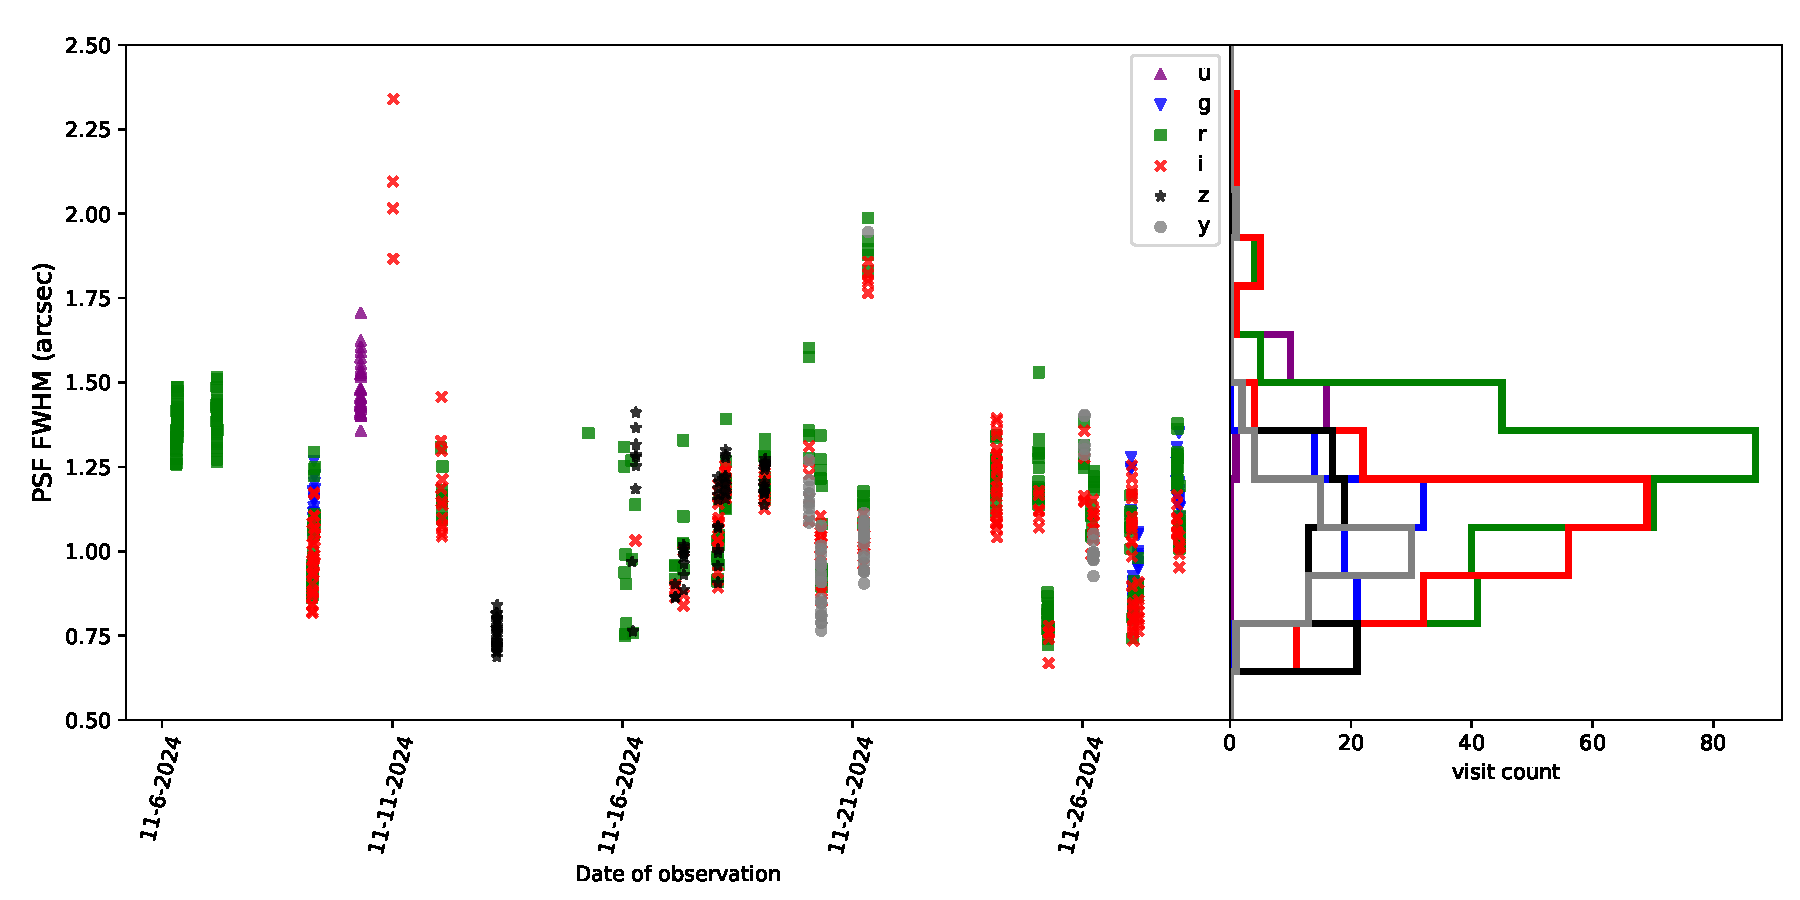
\includegraphics[width=\textwidth]{figures/seeing}
        \caption{\small PSF FWHM as a function of the observed date. Data are from DRP from 2024-11-01 to 2024-11-28.}
        \label{seeing_plot}
\end{figure*}


\begin{table*}
\centering
\begin{tabular}{@{}lccc@{}}
\textbf{Filter} & \textbf{Number of Visits} & \textbf{Mean PSF FWHM} & \textbf{STD PSF FWHM} \\ 
All           & 775                      & 1.12                   & 0.23                  \\
u             & 28                       & 1.49                   & 0.08                  \\
g             & 86                       & 1.07                   & 0.14                  \\
r             & 307                      & 1.18                   & 0.22                  \\
i             & 203                      & 1.09                   & 0.24                  \\
z             & 85                       & 1.01                   & 0.21                  \\
y             & 66                       & 1.04                   & 0.18                  \\ 
\end{tabular}
\caption{Summary of PSF FWHM statistics. Data are from DRP from 2024-11-01 to 2024-11-28.}
\label{tab:psf_summary}
\end{table*}


\textbf{On PSF Modeling:}

Two different PSF models are currently used in the DM pipeline: PSFEx, which provides a fast preliminary PSF estimation, and Piff, used later in the pipeline for more accurate PSF modeling. During the initial data collection with LSSTComCam and AOS testing, most in-focus star shapes exhibited doughnut-like patterns, reflecting residual optical aberrations that had not yet been corrected. This specific form of asymmetry posed challenges for PSF modeling and was not typical. Interestingly, Piff, despite being the more advanced model, struggled to handle the large, non-symmetric PSFs compared to PSFEx. Fig. \ref{growth_plot} shows how we were able early in the observation to constrain the PSF.


\begin{figure*}
        \centering
        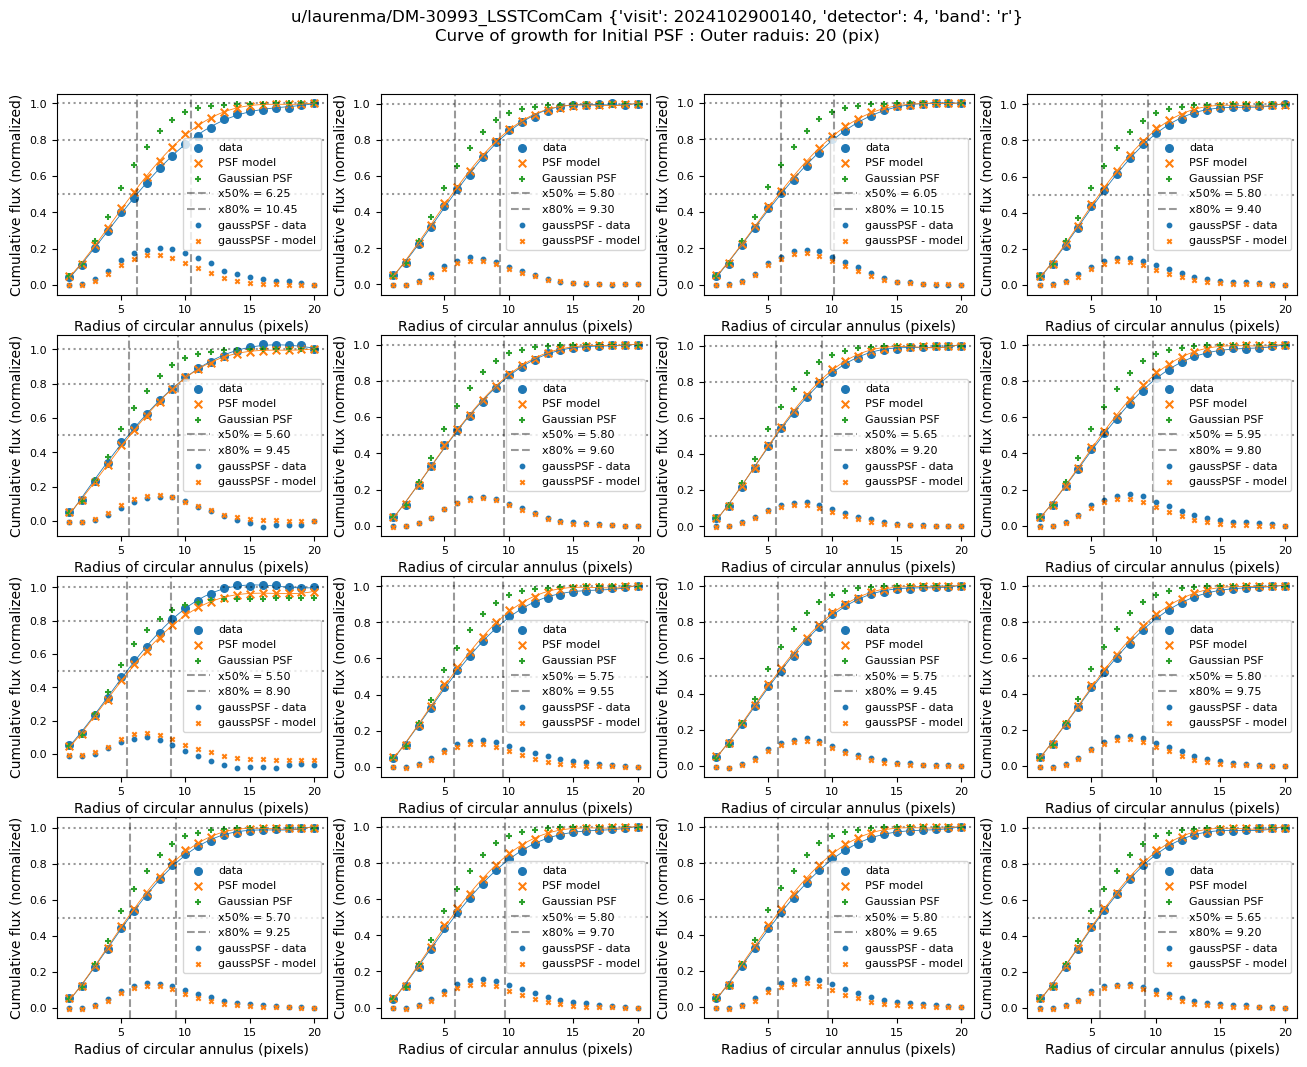
\includegraphics[scale=0.2]{figures/curveOfGrowth_pfsex_u_laurenma_DM-30993_LSSTComCam_2024102900140_4}
        \caption{\small Growth curves of the PSF compared to its model (PSFex here)  in the early data taken with LSSTComCam. }
        \label{growth_plot}
\end{figure*}



However, as the AOS system improved image quality and produced more symmetric PSFs, we observed behavior more consistent with expectations for both PSFEx and Piff. 
Analysis of second-moment reconstructions shows that PSFEx has a systematic offset in size reconstruction compared to Piff, which aligns with observations from DES. Overall, Piff demonstrates better PSF reconstruction, as illustrated in Fig. \ref{DT_plot}. 

\begin{figure*}
        \centering
        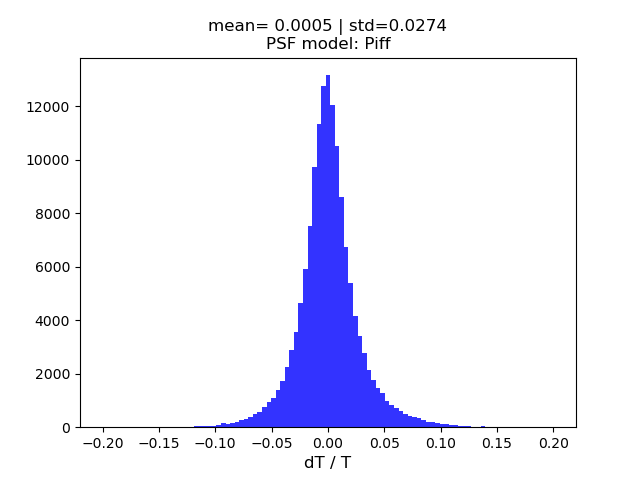
\includegraphics[scale=0.47]{figures/0_dT_1d_Piff}
        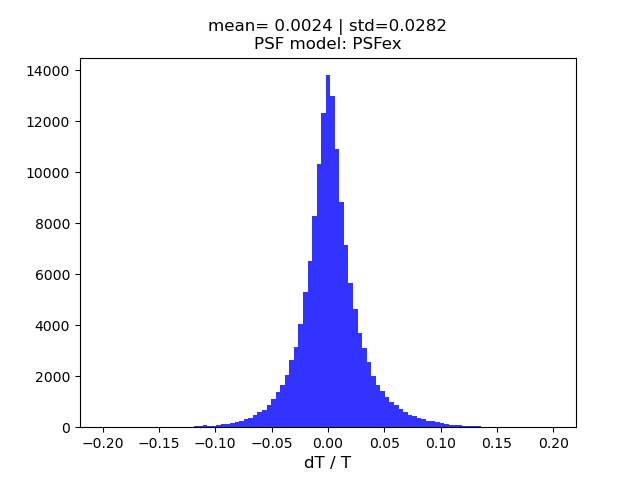
\includegraphics[scale=0.47]{figures//0_dT_1d_PSFex}
        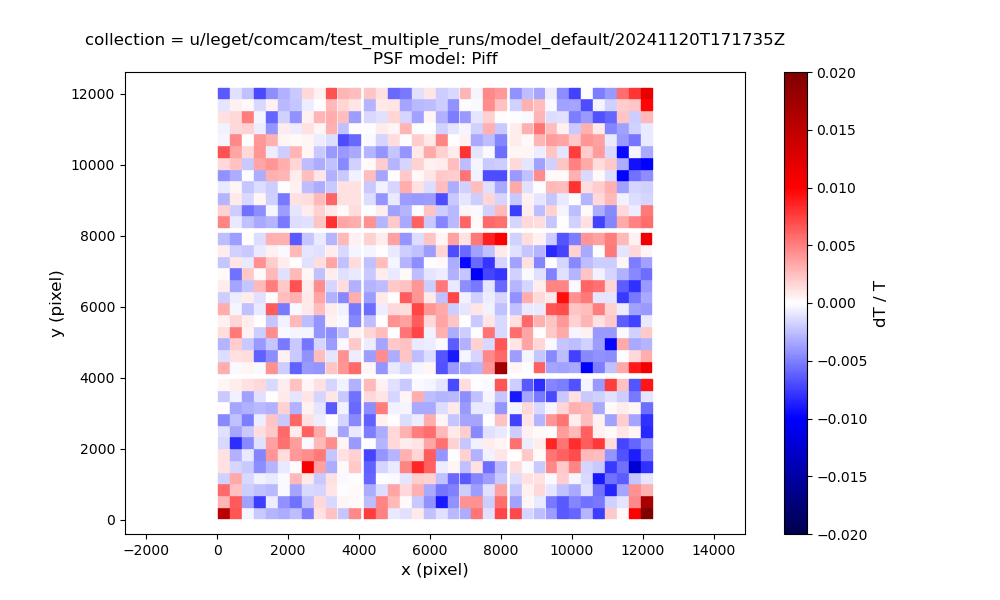
\includegraphics[scale=0.3]{figures/0_dT_2d_Piff}
	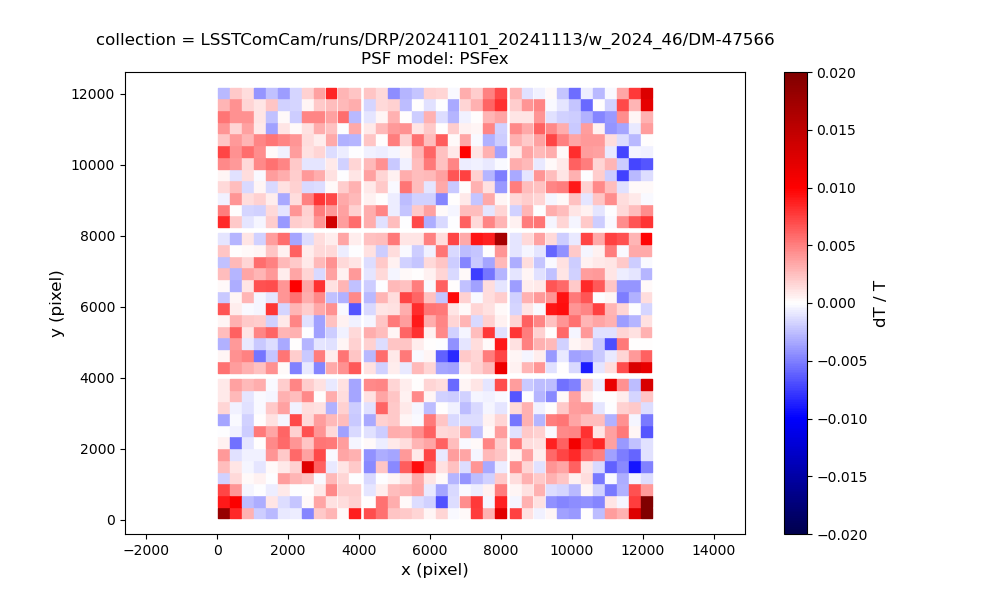
\includegraphics[scale=0.3]{figures/0_dT_2d_PSFex}
        \caption{\small Size residuals for Piff and PSFex (1d distribution and 2d average across visits). Piff has no offset and smaller scatter. Both panels 
        exhibit spatial structure across the focal plane, based on spatial averages across all science visits. The PSF is modeled per CCD in pixel coordinates 
        using a second-order polynomial for interpolation. The observed structure is unlikely to result from atmospheric or dome effects, given that this plot 
        represents an average across visits. Instead, it likely reflects spatial variations not captured by the second-order polynomial interpolation, such as 
        optical aberrations or sensor anomalies.}
        \label{DT_plot}
\end{figure*}


\textbf{On Understanding PSF Physics:}


With LSSTCam, we aim to leverage wavefront sensor data to estimate the optical system's current state and model the optical contribution to the PSF, ultimately building a physical PSF model. During AOS testing with ComCam, the optical state was estimated using out-of-focus images to predict the optical contribution to PSF shape. A ray-tracing analysis showed that the optics fitted from these images could predict the PSF shape, providing strong evidence that a physical PSF model could be developed for LSSTCam (See  Fig. \ref{PSF_plot})


\begin{figure*}
        \centering
        
\includegraphics[scale=0.47]{figures/PSF_plot}
        \caption{\small Plots are located at s3df in this repository: /sdf/group/rubin/shared/notebooks/leget/DM-47689.  In-focus star and prediction from the ray tracing on predicting PSF shape.}
        \label{PSF_plot}
\end{figure*}